\chapter{GPU构架及CUDA编程技术}
\section{GPU:大规模并行处理器}GPU最开始是为图形渲染而设计的,它负责处理计算机系统的图形渲染任务。
图形渲染操作具有高度数据并行性,一般要对大量图形元素执行相同的操作,因此非常适合在SIMD(单指令多数据)
型并行构架上并行实现。其另一个特点是对每个元素执行的操作较为简单因此适合于细粒度并行。
GPU的设计正体现了图形处理的这些特点,现代GPU包含大量功能较为简单的处理单元和存储控制单元,
通过在这些处理单元同时执行大量线程可以达到掩藏访存延迟的目的,
这与CPU设计思想不同,CPU核心只有一个具有复杂控制功能的处理单元,
并用大缓存来掩藏访存延迟。
图\ref{fig:gpu_cpu_arch}所示为CPU和GPU的晶体管使用情况。
\begin{figure}[htpb]
  \centering
  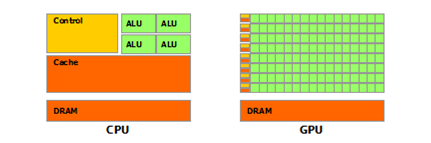
\includegraphics[]{img/gpu_cpu_arch}
  \caption{GPU和CPU的晶体管结构 \footnotesize 来源:NVIDIA}
  \label{fig:gpu_cpu_arch}
\end{figure}
由于图形渲染任务的并行性,设计GPU时可以简单的通过增加晶体管数量来扩充其计算性能和存储带宽。
图\ref{fig:performance}和\ref{fig:bandwidth}所示为CPU和GPU计算速度和存储发展情况比较。
可以看出,目前主流的GPU比同期CPU计算速度和存储带宽都高出很多倍。

\begin{figure}[htb]
  \centering
  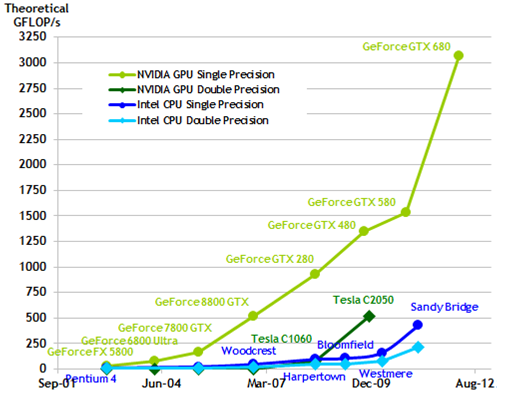
\includegraphics[]{img/performance}
  \caption{GPU和CPU的每秒浮点运算次数 \footnotesize 来源:NVIDIA}
  \label{fig:performance}
\end{figure}

\begin{figure}[htb]
  \centering
  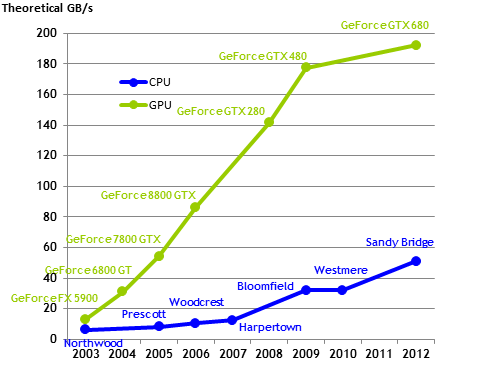
\includegraphics[]{img/bandwidth}
  \caption{GPU和CPU的的存储带宽 \footnotesize 来源:NVIDIA}
  \label{fig:bandwidth}
\end{figure}

\section{GPU构架}\label{sec:gpu_arch}
图形显卡在硬件上主要由GPU芯片、显存以及PCI总线组成。目前市场上主流的显卡主要由
两家公司设计\---NVIDIA和AMD,二者在结构和功能部件名称上存在一些差别。
由于本文研究的是NVIDIA公司的CUDA技术构架下的GPGPU
编程,所以后文对GPU结构和功能的介绍均以NVIDIA公司的显卡为例,
具体的,我们将使用NVIDIA公司的高端显卡\---Tesla C1060。

GPU芯片上集成了大量处理单元,是显卡的计算功能部件。Tesla C1060 显卡使用的是一个GT200 GPU核心。
核心中的处理单元按两层结构组织\---多处理器(SM)和流处理器(SP),其中一个SM包含多个SP。
GT200核心上有30个SM,每个SM包含有8个SP,因此一共是240个SP。每个SP有一个单精度计算单元,每个
SM拥有一个双精度计算单元。SP工作频率为1296MHz,SP每个时钟周期能执行3次单精度浮点数操作,
每个双精度计算单元每个时钟周期能执行2次双精度浮点数操作。因此GT200核心理论单精度计算能力为
$240\times 1296\text{(MHz)}\times 3\text{(flops)} \approx 933\text{Gflops}$, 双精度计算能力为
$30\times 1296\text{(MHz)}\times 2\text{(flops)} \approx 78\text{Gflops}$。 
GT200核心的双精度计算能力是单精度的$1/12$,因此其计算性能的优势主要体现在单精度浮点数计算上。
在NVIDIA公司后来推出的Fermi构架和最新推出的Kepler构架的GPU上,双精度浮点数计算速度大为改善,
可以达单精度的$1/2$。
%每个SM上有16KB的共享存储器(shared memory),
%它是一种高速存储器,SP访问它只有2-4个是·
值得指出的是,虽然SP是GPU核心实际的计算单元,但由于SP没有独立的寄存器和取指、调度单元,
所以SP并不是一个独立的类似CPU的执行单元。

显存作用类似于CPU构架中的内存,是GPU主要存储器。Tesla C1060 显存大小为4GB。多处理器通过
8个存储控制器与显存相连,每个存储控制器位宽为64bit,所以显存总位宽是$8\times 64\text{bit}=512\text{bit}$。
存储单元工作频率为2214MHz,理论外部存储带宽为$512\times 2214\text{Mhz}\approx142\text{GB/s}$。和CPU相同,
由于存在较大的访存延迟,GPU的外部存储带宽往往是程序性能的一个限制因素。

PCI-E总线是显存与主板芯片组的数据通道,总线带宽根据所采用PCI-E规范版本及通道数量不同而有所差异。
通常能提供上下各数GB/s的带宽。总线带宽比显存外部带宽带宽低得多,容易成为程序性能的瓶颈,
所通常要尽量减少CPU主存与GPU显存之间的频繁地数据传输。

\section{CUDA编程模型}
CUDA技术的提出,大大简化了通用GPU计算程序的开发。在CUDA技术提出之前,要想利用GPU做通用计算,
编程人员必须掌握计算机图形API和图形硬件细节,并将自己的应用程序按照计算机图形学里面的概念
来描述和编码,这种方式繁琐而不自然。 2007年,NVIDIA推出了CUDA技术,与传统GPGPU不同,CUDA将
图形学API隐藏起来,直接C语言基础上扩展,它允许编程者自己编写一种类似普通C函数的\textit{Kernel}函数
在SP上执行,从而利用GPU的大规模并行计算能力。另外它还提供线程执行控制、存储器管理等功能并以运行时库函数
的方式供CPU上执行的普通函数调用。下面介绍CUDA技术中的几个关键概念。
\begin{myDescription}
\item[Host与Device] 一个完整的CUDA程序包含在CPU执行的部分和在GPU上执行的部分。CPU端被称作\textit{Host}端,
  GPU端被称为\textit{Device}端。Host端运行的代码是标准的C语言(或Fortran、Python等其它语言),而Device端
  运行的代码是由扩展的C语言编写的,并被封装在一个在声明时由\verb+__global__+修饰的函数中,这种
  函数被称作\textit{Kernel}。当Host端程序运行到要调用Kernel时,编译好的Kernel代码被装载到Device端,开始
  由GPU核心执行。图\ref{fig:cuda_program}示例为CUDA程序的执行过程。
  \begin{figure}[htpb]
    \centering
    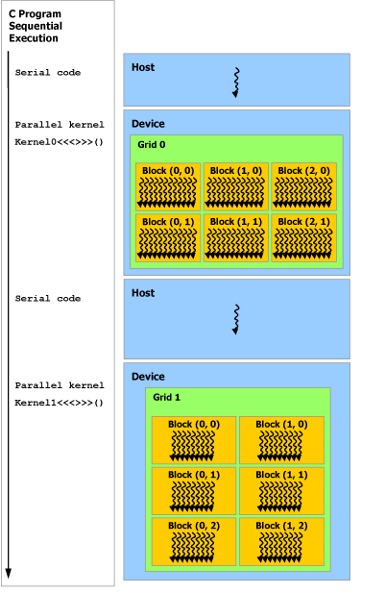
\includegraphics[]{img/cuda_program}
    \caption{CUDA程序执行流程 \footnotesize 来源:NVIDIA}
    \label{fig:cuda_program}
  \end{figure}

\item[线程] 
线程(thred)是CUDA的核心概念,它是与流处理器SP相对应的逻辑
上的概念,可以理解为GPU代码的一条逻辑执行主线。
在已经充分掩藏了访存延迟的情况下,GPU核心里面的每个SP都同时运行着一个线程。
这种线程的粒度相对于CPU上的线程而言非常小,并且通常没有复杂的逻辑判断分支执行路径。


\item[Block与Grid] 运行Kernel的线程按层次被组织为线程块\textbf{Block}与线程块网格\textbf{Grid}。
  通常整个求解域被映射到一个Grid上,并被划分为细小的单元,Grid中的每个线程负责处理一个单元。
  Grid中的线程又按划分为Block,划分方式可以是一维、二维或者三维,相应的Block也可以是一维、二维或三维的。
  Grid和Block的大小(即Grid各维度上Block的数量和Block各维度上线程数量)分别由\verb+dim3+类型的参数指定。这种变量
  有三个整数分量,分别指定Grid或Block在各维度上元素的个数(二维可以看做特殊的三维情况,及第三个分量为1)。
  在调用Kernel时指定这些参数,这些参数并以内建全局变量的形式出现在Kernel函数中,分别为\verb+gridDim+
  和\verb+blockDim+。在Kernel中还有两个\verb+uint3+类型的局部变量\--- \verb+blockIdx+和\verb+threadIdx+,
  它们也有三个整数分量。\verb+blockIdx+记录当前线程所属Block在Grid中的位置,\verb+threadIdx+记录当前线程
  在其Block中的位置。每个线程可以根据这些变量确定其在grid中的位置,进而确定其所处理的数据在显存中的位置。
  位于同一个Block中的线程共享部分高速存储器\---共享内存。CUDA还提供\verb+__syncthreads()+函数来实现块内线程同步。
  通过共享内存和线程同步,CUDA提供了一种简单的线程间通信能力。Block中的线程又隐式的被划分为若干个\textit{wrap},
  wrap的概念在CUDA源程序中没有体现,但线程执行和访存时是按wrap为单位进行的。
\end{myDescription} 

代码1提供一个完整的CUDA程序实例\---矩阵$\bm A$和$\bm B$的求和运算,上述各种概念在其中已有体现。
\begin{Code}
\begin{lstlisting}
#define N 1024
#define BX 16
#define BY 16
float A_h[N][N], B_h[N][N],  C_h[N][N];//Host`端存数组` 
float *A_d, *B_d, *C_d;//`Device端数据指针`
//Kernel`函数定义`
__global__ void
 matrixAdd(float A[N][N], float B[N][N], float C[N][N]) 
{
	int x = blockId.x*blockDim.x + threadIdx.x;
	int y = blockId.y*blockDim.y + threadIdx.y;
	C[y][x] = A[y][x] + B[y][x];
}  
int main()
{
	...
	//Host`端初始化`A_h, B_h
	...
	//Device`分配显存存储Device端数据`
	cudaMalloc((void**)A_d, sizeof(float)*N*N);
	cudaMalloc((void**)B_d, sizeof(float)*N*N);
	cudaMalloc((void**)C_d, sizeof(float)*N*N);
	//`拷贝Host端数据到Device端`
	cudaMemcpy(A_d, A_h, cudaMemcpyHostToDevice);
	cudaMemcpy(B_d, B_h, cudaMemcpyHostToDevice);
	dim3 GRID(BX, BY);//`定义Grid尺寸`
	dim3 BLOCK(N/BX, N/NY);`定义Block尺寸`
	//`调用`Kernel
	matrixAdd<<<GRID, BLOCK>>>(A_d, B_d, C_d);
	//`将结算结果`C`拷回Host端`
	cudaMemcpy(C_h, C_d, cudaMemcpyDeviceToHost);
	...
	//Host`端的后续操作`
	...
	return 0;
} 
\end{lstlisting}  
\caption{一个实现矩阵相加(C=A+B)的CUDA程序}
\end{Code}


%\section{存储器类型}
和Host端类似,在Device端也存在各种不同的存储器类型。它们的大小、访问开销各不相同。合理的使用用它们
是提高CUDA程序性能的关键,这里我们介绍常用的几种存储器类型。
\begin{myDescription}
\item[全局存储器] 
全局存储器(global Memroy)位于显存并占据了显存的绝大多数空间,
功能类似于Host段的主存,用来存贮主要的计算数据,如LBM中的分布函数、宏观量等。全局存储器通
过调用\texttt{cudaMalloc}来分配,通过调用\texttt{cudaMemcpy}实现全局内存与Host内存之间的数据传输。
全局内存的访问开销相对其他类型的存储器非常大,通常有几百个时钟周期延迟。同一个wrap中的线程
访问全局存储器时,若访存地址满足对齐要求并且相邻线程访问的地址连续,会被合并为一次访问请求,
只需要进行一次数据传输,否则会及进行多次数据传输,显存带宽会大幅下降,在早期的GPU上,这一效应
尤为明显。

\item[寄存器] 寄存器(register)是GPU片上的一种高速存储器,Kernel函数声明的临时变量通常就是这种类型。
在GT200核心中,每个SM寄存器大小为16KB,SM同时为多个线程维护一份寄存器,所以每个线程分配到的寄存器
数量非常有限。若Kernel中寄存器用量超过其上限,数据就会被存储到局部存储器,后者访存开销相当大。

\item[共享内存] 共享存储器(shaared memory)是位于GPU芯片上的一种高速存储器,几乎没有访存延迟,
它可以被同一个Block中的所有线程访问。共享内存数量较少,是一种稀缺资源,如GT200核心中每个SM的
的共享内存数量为16KB。在Kernel函数中通过\texttt{\_\_shared\_\_}修饰声明。

\item[常数存储器] 常数存储器(constant memory)是一种只读的存储器,
  通常用来存储少量计算参数。常数存储器也较少,GT200核心只有64KB大小。

\item[局部存储器] 局部存储器位于显存,当寄存器用完时会自动被使用,访问开销与全局存储器相同。
\end{myDescription}

\section{CUDA程序优化的基本原则}\label{sec:cuda_principle}
为充分利用GPU提供的大量处理器和存储带宽,设计和优化程序时要遵守一些基本原则,否则
GPU的实际性能会大为降低,下面列出一些常见的要求
\begin{itemize}
  \item Block大小为应该是32的整数倍;
  \item 控制Kernel汇总共享内存和寄存器用量,保证SM上至少
    能容纳2个活动的Block和6个活动的wrap,否则不能充分
    掩藏全局存储器访问延迟;
  \item 合理选择Block尺寸,此要求通常与上一条要求相互矛盾,
    实际设计时要根据计算实验来确定最优Block尺寸;
  \item 尽量保证访存满足地址对齐和连续的要求。
\end{itemize}

\section{小结}
本章前半部分介绍了GPU的基本构架和相应结构的功能,比较了其与CPU构架的差异,
并揭示了GPU之所以具有大规模并行能力的底层原因。本章后半部分主要主要介绍了
CUDA技术的基本概念,涉及到了CUDA技术的线程层次结构和存储器类型,理解这些
基本概念以及各种存储器的差异和使用要求是设计出高效率CUDA程序的前提。最后
我们列出了CUDA程序优化的基本原则,我们将在后面章节根据这些原则的指导设计
和优化LBM模拟的CUDA程序。

